\chapter{Transformée de Fourier}

\section{Généralités, Définitions et Propriétés}

\subsection{Les ensembles $L^1(\mathbb{R})$ et $L^2(\mathbb{R})$\label{L2}}
On admettra l'existence des ensembles de fonctions suivants :
\begin{definition}
L'ensemble $L^1(\mathbb{R})$ désigne les fonctions définies et intégrables sur $\mathbb{R}$ c'est à dire : 
$$L^1(\mathbb{R})=\left\{s:\mathbb{R}\rightarrow\mathbb{C},\int_\mathbb{R}|s(t)|dt<+\infty\right\}.$$

De\ fa\c{c}on\ analogue, l'ensemble $L^2(\mathbb{R})$ désigne les fonctions définies et de carré intégrable sur $\mathbb{R}$, c'est à dire : 
$$L^2(\mathbb{R})=\left\{s:\mathbb{R}\rightarrow\mathbb{C},\int_\mathbb{R}|s(t)|^2dt<+\infty\right\}.$$ 
\end{definition}

$L^2(\mathbb{R})$ correspond également à l'ensemble des signaux d'énergie finie, $\int_\mathbb{R}|s(t)|^2dt<+\infty$ représentant l'énergie du signal $s$.\\

$L^1(\mathbb{R})$ et $L^2(\mathbb{R})$, munis de l'addition usuelle des fonctions et de la multiplication par un scalaire, sont des espaces vectoriels.\\

On définit sur l'ensemble $L^2(\mathbb{R})$ un produit scalaire pour s et $\sigma$ dans $L^2(\mathbb{R})$ par :\
$$\langle s,\sigma\rangle=\int_\mathbb{R}s(t)\overline{\sigma}(t)dt.$$

\begin{definition}\label{pp}
On dit que deux fonctions s et $\sigma$ de $L^2(\mathbb{R})$ sont orthogonales
si et seulement si $$\int_\mathbb{R}s(t)\overline{\sigma}(t)dt=0.$$ \
\end{definition}

La norme associée à ce produit scalaire est définie pour
$s\in L^2(\mathbb{R})$ par :
$$\|s\|_2=\sqrt{\langle s,s\rangle}=\sqrt{\int_\mathbb{R}|s(t)|^2 dt}. $$
\\

Sur l'espace $L^1(\mathbb{R})$ on définit aussi une norme pour
$s\in L^1(\mathbb{R})$ par :
$$\|s\|_1=\int_\mathbb{R}|s(t)|dt. $$

On remarque, de la même fa\c{c}on que dans le cas des fonctions périodiques , pour ces deux normes, que la norme de $s$ peut être nulle sans que $s$ soit nulle (par
exemple si $s$ est nulle sauf en un nombre fini de points). Pour obtenir une
vraie norme, on va dire qu'une fonction est nulle presque partout lorsque 
l'intégrale de la valeur absolue de cette fonction est nulle, c'est à dire :

\begin{definition}\label{pp}
$$s\stackrel{p.p.}{=}0~~~\text{(presque partout)}~~~\Longleftrightarrow~~~
\dpy \int_\mathbb{R}|s(t)| dt=0.$$\\
$$s_1\stackrel{p.p.}{=}s_2~~~\text{(presque partout)}~~~\Longleftrightarrow~~~
\dpy s_1-s_2\stackrel{p.p.}{=}0~~~$$ 
\end{definition}
~~\\
 
\subsection{Définitions}
On considère une fonction $s$, à valeurs réelles ou complexes, élément de $L^1(\mathbb{R})$. 
\begin{definition} On appelle transformée de Fourier du signal s la fonction F[s] définie par :
$$F[s](f)=\int_\mathbb{R}s(t)e^{-2i\pi ft}dt$$
\end{definition}
$F[s]$ est aussi notée $S$.
~~\\

Pour un signal périodique de période $T_0$, la série de Fourier associée à un signal $s$ s'interprète comme la décomposition de ce signal sur l'ensemble dénombrable des harmoniques $nf_0$, $n\in\mathbb{Z}$, par l'intermédiaire des exponentielles trigonométriques. Pour un signal de $L^1(\mathbb{R})$, on peut voir la transformée de Fourier comme la décomposition du signal $s$ sur les harmoniques $f$, $f\in\mathbb{R}$; l'intégrale est obtenue intuitivement par un passage à la limite à partir des séries de Fourier en faisant tendre la période $T_0$ vers +$\infty$.

\subsection{Propriétés}

\begin{prot} La transformée de Fourier est une application linéaire, c'est-à-dire: 
$$\forall u, v \in L^1(\mathbb{R}),\ \forall\lambda \in \mathbb{C},\ F[\lambda u+v]=\lambda F[u]+F[v]$$ 
\end{prot}
~~\

\begin{prot} La transformée de Fourier de s est une fonction continue et bornée, en effet on a : 
$$\forall f \in \mathbb{R}~~ |{F[s]}(f)|\leq \|s\|_1$$ 
et $F[s](f)$ a pour limite 0 quand $f$ tend vers $\pm \infty$.
\end{prot}
~~\\
Cette dernière propriété sera admise.
~~\\

\begin{prot} Soit s $\in L^1(\mathbb{R})$, notons $s_-$ la fonction $t\rightarrow s(-t)$, alors
$$F[s_-](f)=F[s](-f)$$ 
\end{prot}
~~\

\begin{prot} Soit s $\in L^1(\mathbb{R})$, alors
$$F[\overline{s}](f)=\overline{F[s](-f)}$$ 
\end{prot}
~~\

Selon la parité de la fonction $s$, on peut, à partir des deux propriétés précédentes, simplifier l'expression de la transformée de Fourier :
\begin{prot}
Si $s$ est une fonction paire, alors :
$$F[s](f)=2\int^{+\infty}_{0}s(t)cos(2\pi ft)dt$$
Si $s$ est une fonction impaire, alors :
$$F[s](f)=2i\int^{+\infty}_{0}s(t)sin(2\pi ft)dt$$\end{prot}
~~\\

\begin{prot} 
Soit s $\in L^1(\mathbb{R})$, alors, en notant $H_a$ l'application $t\rightarrow at$ (homothétie\ de\ vecteur a), on a
$$F[{s\ o\ H_a}](f)=\frac{1}{|a|}\ F[s](\frac{f}{a})$$ 
\end{prot}
~~\\

\begin{prot} Théorème du retard
~~\\
Soit s $\in L^1(\mathbb{R})$, alors, en notant $U_a$ l'application $t\rightarrow t-a$ (translation de vecteur a), on a
$$F[\ s\ o\ U_a\ ](f)=e^{-2i\pi fa}\ F[s](f)$$ 
\end{prot}
~~\

\begin{prot} 
Soit s $\in L^1(\mathbb{R})$, alors, en notant $e^{2i\pi f_0.}$ la fonction $t\rightarrow e^{2i\pi f_0t}$, on a
$$F[e^{2i\pi f_0.}\ s](f)=F[s](f-f_0)$$ 
\end{prot}
~~\

\subsection{Exemples}
\subsubsection{Signal porte}
Soit $s$ la fonction définie sur $\mathbb{R}$ par : $\Pi(t)=1$ pour $t\in[-1/2,1/2[$,
$\Pi(t)=0$ sinon. On dit que $\Pi$ est un signal porte. La fonction $\Pi$ est paire et est représentée figure \ref{Porte} .
%
%pour numeroter les figures j'utilise label
%et caption pour donner un titre
% le [htbp] force latex a mettre la figure a l'endroit donne
%
\begin{figure}[htbp]
\centering
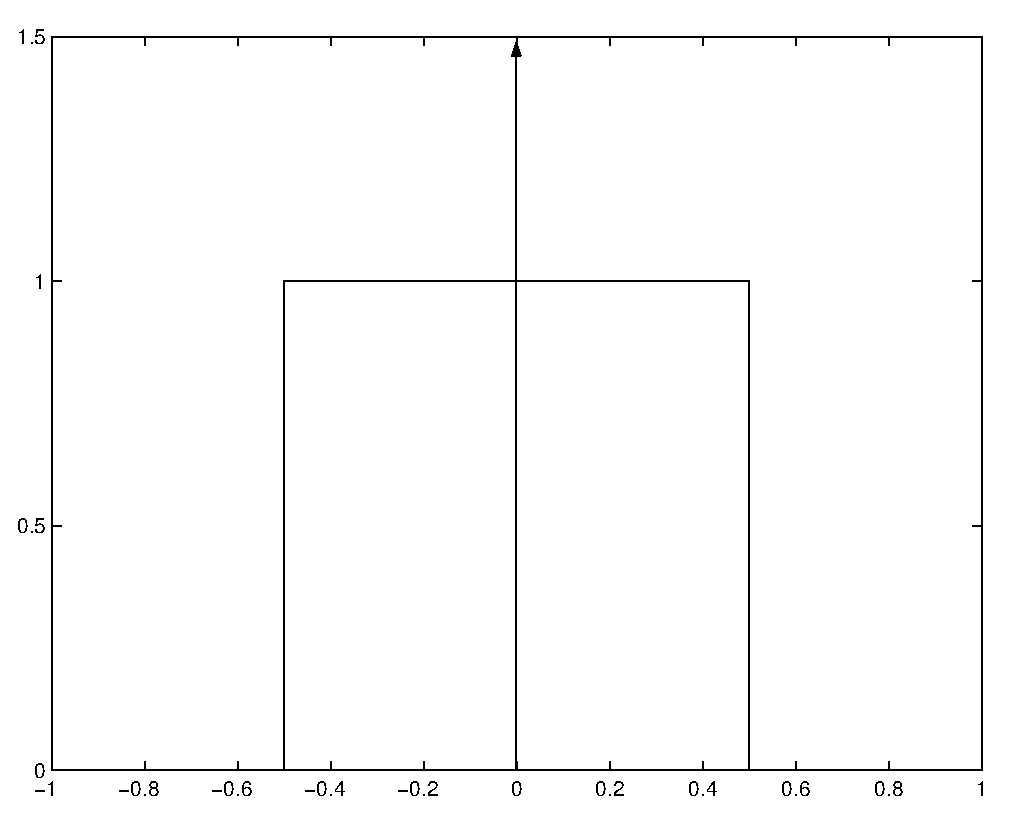
\includegraphics[width=6cm]{porte.eps}
\caption{Signal Porte}
\label{Porte}
\end{figure}
\begin{figure}[htbp]
\centerline{
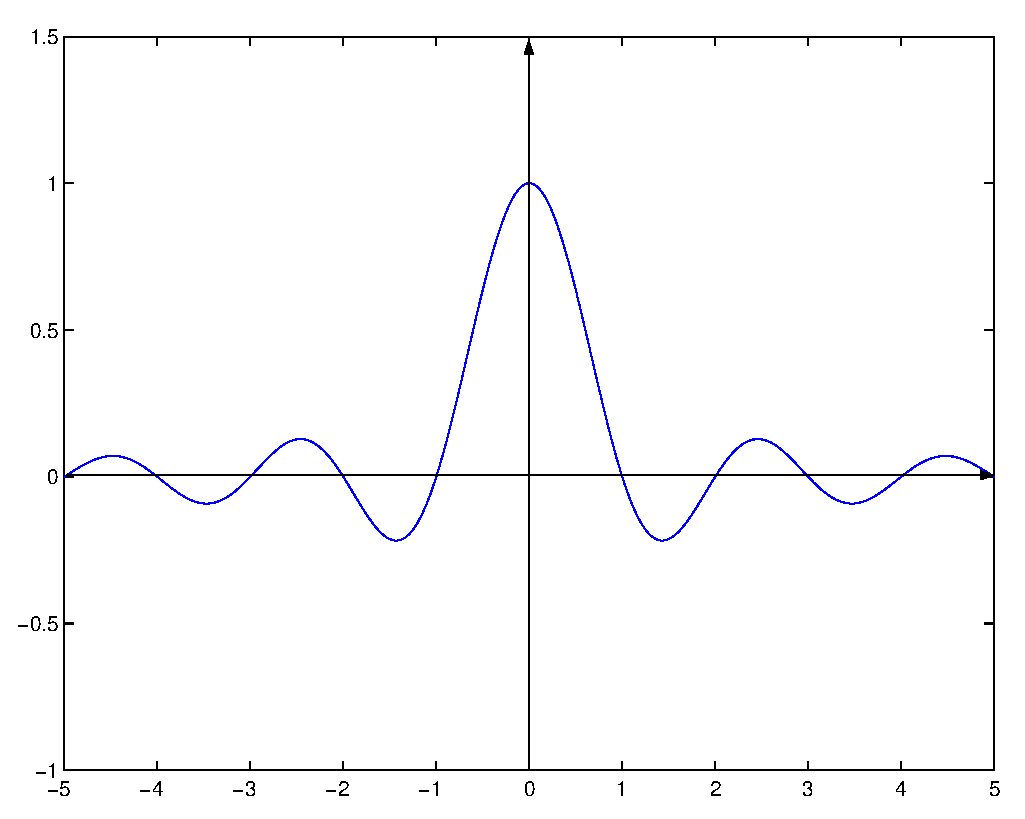
\includegraphics[width=6cm]{sinca.eps}}
\caption{Transformée de Fourier du signal porte}
\label{sinca}
\end{figure}

Le calcul de sa transformée de Fourier donne un sinus cardinal (cf. figure \ref{sinca} ):

$$F[s](f)=\frac{sin(\pi f)}{\pi f}= sinc(f)$$


\subsubsection{Signal triangulaire}
Soit $\sigma$ la fonction définie sur $\mathbb{R}$ par $\sigma(t)=(1 -2|t|)\Pi (t)$ . La fonction $\sigma$ est paire et est représentée figure \ref{triang}.
\begin{figure}[htbp]
\centerline{
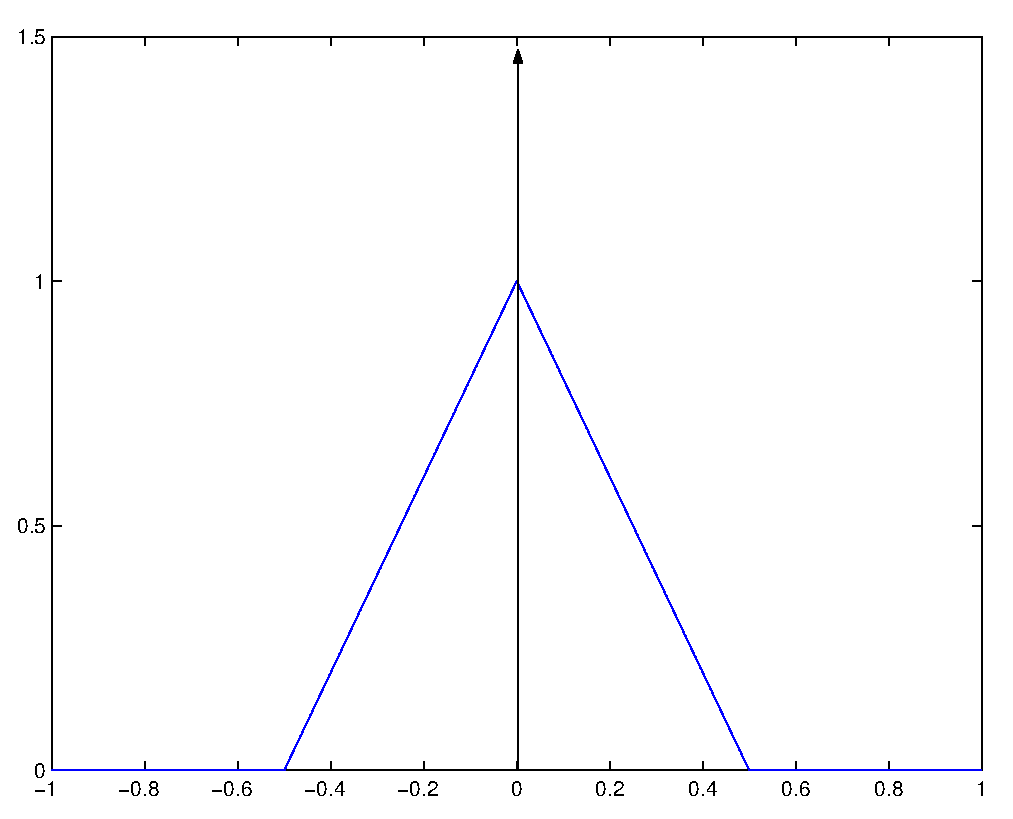
\includegraphics[width=6cm]{triang.eps}}
\caption{Signal triangulaire}
\label{triang}
\end{figure}
\begin{figure}[htbp]
\centerline{
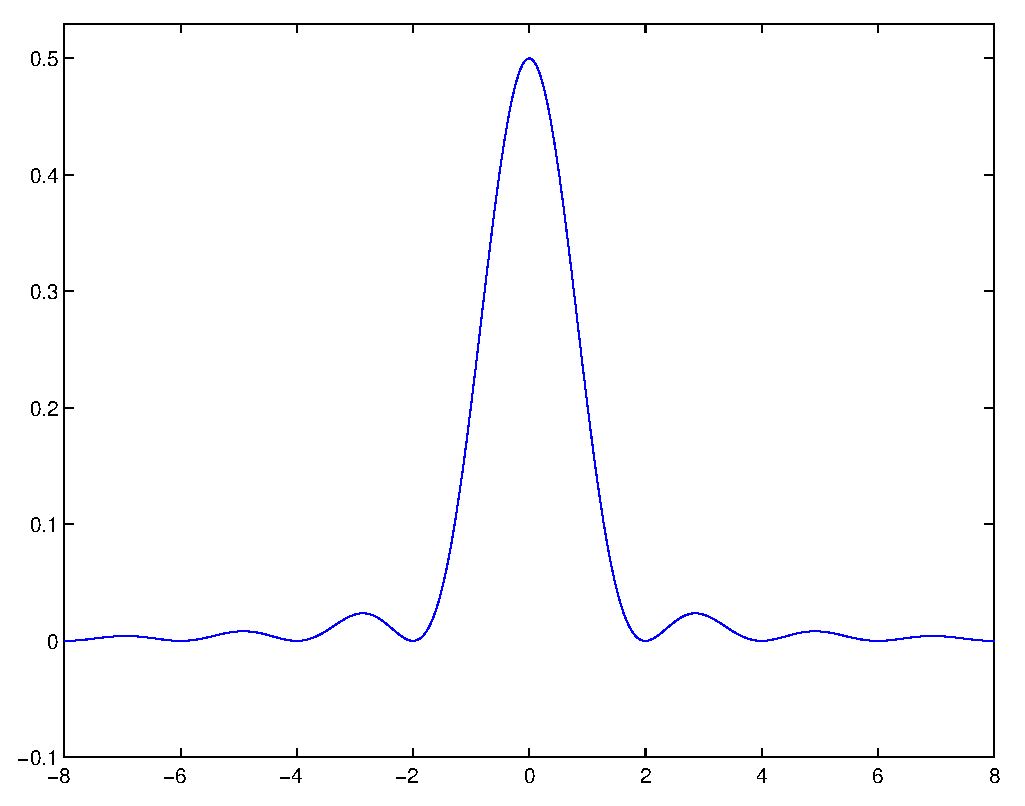
\includegraphics[width=6cm]{sinca2.eps}}
\caption{Transformée de Fourier du signal triangulaire}
\label{sinca2}
\end{figure}

Le calcul de sa transformée de Fourier donne (cf. figure \ref{sinca2}) :

$$F[s](f)=2{[\frac{sin(\pi f/2)}{\pi f}}]^{2}$$

\subsubsection{Signal gaussien}
Soit $s$ la fonction définie sur $\mathbb{R}$ par : $s(t)=e^{-t^2}$ pour $t$ réel. $s$ est appelé signal gaussien. La fonction $s$ est paire et est représentée figure \ref{gauss} .
\begin{figure}[htbp]
\centerline{
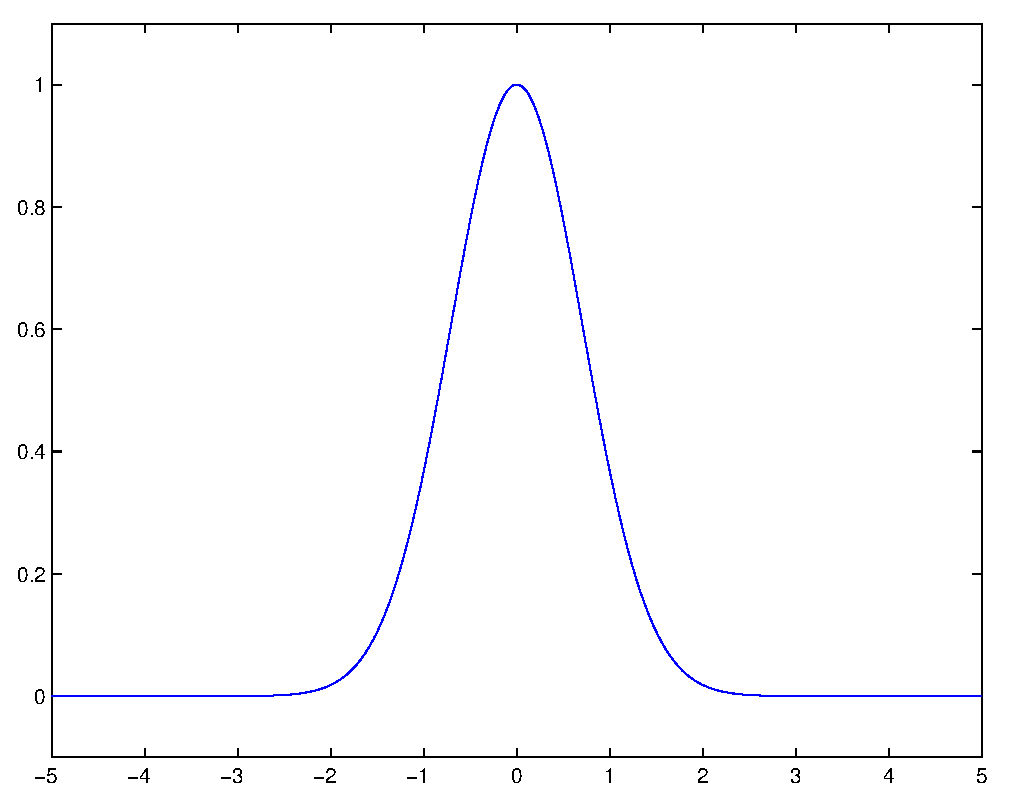
\includegraphics[width=6cm]{gauss.eps}}
\caption{Signal gaussien}
\label{gauss}
\end{figure}
\begin{figure}[htbp]
\centerline{
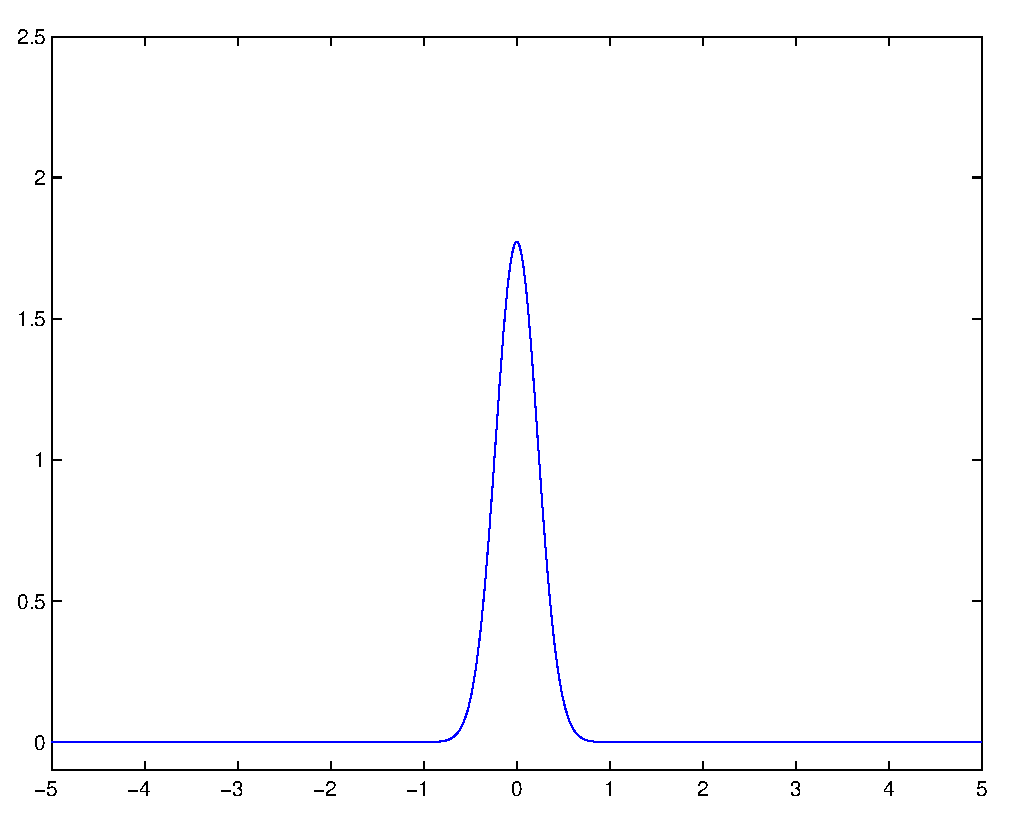
\includegraphics[width=6cm]{gaussfou.eps}}
\caption{Transformée de Fourier du signal gaussien}
\label{gaussfou}
\end{figure}

Le calcul de sa transformée de Fourier donne un signal lui aussi gaussien (cf. figure \ref{gaussfou} ):

$$F[s](f)=\sqrt{\pi}e^{-\pi^2f^2}$$

Ce calcul sera effectué en TD.


\section{Dérivation}

\subsection{Transformée de Fourier d'une dérivée}

\begin{thme}\label{thder}
Soit une fonction s $\in L^1(\mathbb{R})$ dérivable, dont la dérivée $s\ '$ est aussi dans $L^1(\mathbb{R})$, alors,
$$F[s\ '](f)=2i\pi f F[s](f)$$
Si $s$ est dérivable p fois et a ses dérivées jusqu'à l'ordre p dans $L^1(\mathbb{R})$, alors
$$F[s^{(p)}](f)={(2i\pi f)}^p F[s](f)$$
\end{thme}
La démonstration de ce théorème repose sur des intégrations par parties et le fait que $s$ et ses dérivées successives tendent vers 0 à l'infini. En effet, on admettra que toutes les fonctions qui sont éléments de $L^1(\mathbb{R})$ tendent vers 0 en $\pm\infty$. 
~~\\
\begin{rmq}
on a la propriété :
$$|F[s](f)|\leq \frac{\left\|s^{(p)}\right\|_{1}}{{(2\pi f)}^p}$$
\end{rmq}

On peut donc en déduire que $F[s]$ tend vers 0 aussi vite que $\frac{1}{f^p}$ quand $f$ tend vers l'infini. 

\subsection{Dérivée d'une transformée de Fourier}

\begin{thme}
Soit une fonction s $\in L^1(\mathbb{R})$ dérivable, telle que, $\forall p$ entier, l'application $(.)^ps : t\rightarrow t^ps(t)$ soit aussi dans $L^1(\mathbb{R})$, 
~~\\
alors $F[s]$ est dérivable et ses dérivées sont données par :
$$F[s]^{(p)}(f)={(-2i\pi)}^p F[(.)^p s](f)$$
\end{thme}
~~\\
La démonstration de ce théorème repose sur la dérivation sous le signe intégrale qui se justifie par l'appartenance des fonctions à $L^1(\mathbb{R})$. 


\subsection{Convolution}
\begin{definition}
Soit deux fonctions $u$ et $v$ dans $L^1(\mathbb{R})$, on peut définir le produit de convolution de $u$ et $v$ par $$u*v(a)=\int_\mathbb{R}u(a-t)v(t)dt$$
\end{definition}
~~\

\begin{prot} 
Le produit de convolution est commutatif, c'est-à-dire :
$$u*v=v*u$$
\end{prot}
~~\

\begin{prot} 
Le produit de convolution est associatif, c'est-à-dire :
$$(u*v)*w=u*(v*w)$$
\end{prot}
~~\

\begin{prot} 
Si $u$ et $v$ dans $L^1(\mathbb{R})$, alors $u*v \in L^1(\mathbb{R})$ et 
$$\|u*v\|_1\leq \|u\|_1 \|v\|_1$$
\end{prot}
~~\

Cette propriété permet de montrer le résultat suivant:

\begin{prot} 
Si $u_n$ et $v_n$ sont deux suites de $L^1(\mathbb{R})$ qui convergent respectivement pour la norme $\| \|_1$ vers deux fonctions de $L^1(\mathbb{R})$ $u$ et $v$, alors $u_n*v_n$ converge vers $u*v$ dans $L^1(\mathbb{R})$, c'est-à-dire pour la norme de $L^1(\mathbb{R})$.  
\end{prot}
~~\

\begin{prot} 
Si $u$ et $v$ sont dans $L^2(\mathbb{R})$, alors $u*v$ existe et 
$$\forall t \in \mathbb{R}, |(u*v)(t)|\leq \|u\|_2 \|v\|_2$$
\end{prot}
~~\\
Cette propriété se démontre en utilisant l'inégalité de Cauchy-Schwarz.
\\
\begin{rmq}
Si $u$ et $v$ sont dans $L^2(\mathbb{R})$, $u*v$ n'est pas forcément élément de $L^2(\mathbb{R})$.
\end{rmq}
~~\

\begin{prot} 
Soit deux fonctions $u$ et $v$ dans $L^1(\mathbb{R})$, alors
$$F[u*v]=F[u]F[v]$$
Si, de plus, $uv\in L^1(\mathbb{R})$ et $F[u]$ ou $F[v]$ aussi, alors
$$F[uv]=F[u]*F[v]$$
\end{prot}
~~\\

\section{Impulsion de Dirac}
Prenons l'exemple de la fonction $g_h=\gfrac{1}{2h}\text{\tt 1\hspace{-0.14cm}I}_{[-h,h]}\ \text{o\'u}\ \text{\tt 1\hspace{-0.14cm}I}_{[-h,h]}$ est la fonction indicatrice de l'intervalle $[-h,h]$, c'est à dire $\text{\tt 1\hspace{-0.14cm}I}_{[-h,h]}(x)=1~\text{ si}~ x\in[-h,h]~\text{ et}~ \text{\tt 1\hspace{-0.14cm}I}_{[-h,h]}(x)=0~\text{sinon}$.
\begin{figure}[htbp]
  \begin{center}
    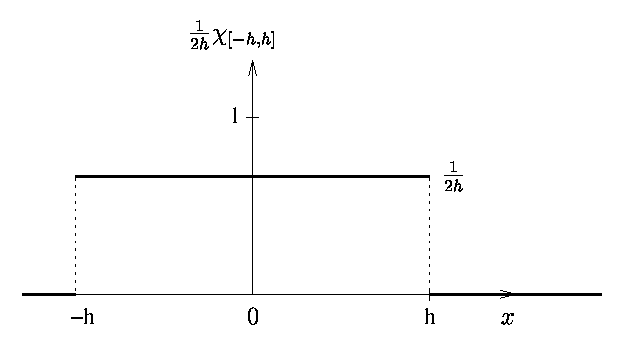
\includegraphics[width=7.2cm]{polyic2_gh.eps}
  \end{center}
\caption{La fonction $g_h$}
\end{figure}
On a 
$$ \int_{-\infty}^{+\infty}g_h(x)dx = 1, \ \ \forall h > 0, $$
Le produit de convolution 
$$ (f*g_h)(x) = \int_{-\infty}^{+\infty}f(x-t)\text{\tt 1\hspace{-0.14cm}I}_{[-h,h]}(t)dt = \gfrac{1}{2h}\int_{-h}^hf(x-t)dt = \gfrac{1}{2h}\int_{-h}^hf(x+t)dt. $$
représente la moyenne de f sur l'intervalle $[x-h, x+h]$. 
%Quand $h$ est petit, $f*g_h(x)$ est proche de $f(x)$ pourvu que $f$ soit continue.
Que devient le produit de convolution $f*g_h$ quand $h$ tend vers $0$ ? L'intervalle sur lequel on fait la moyenne de $f$ autour de $x$ devient de plus en plus petit, et si $f$ est une fonction continue on aura
$$ \lim_{h \rightarrow 0} (f*g_h)(x) = f(x), $$
On se pose alors la question, puisque seule $g_h$ dépend de $h$ de ce qu'est la limite 
%$\lim_{h \rightarrow 0} g_h$.
quand $h$ tend vers 0 de $g_h$.
\begin{figure}[htbp]
  \begin{center}
    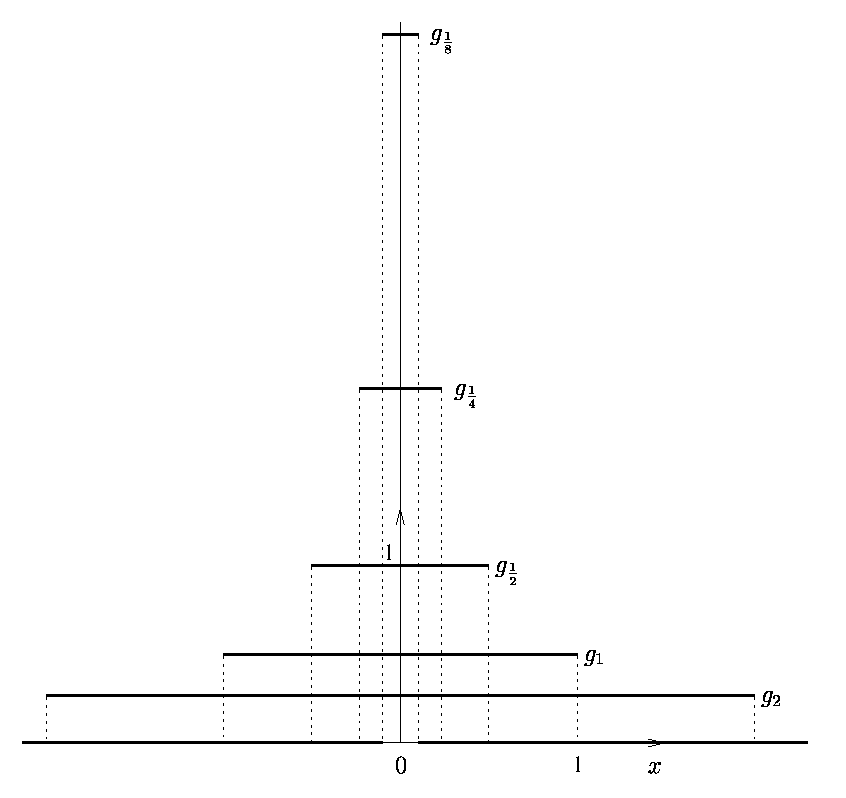
\includegraphics[width=10cm]{polyic2_dirac.eps}
  \end{center}
  \caption{La fonction $g_h$ pour différentes valeurs de $h$} \label{fig:dirac}
\end{figure}
Si cette limite a un sens, alors la ``fonction'' limite, que l'on note $\delta_0 = \ds \lim_{h \rightarrow 0} g_h$ est l'élément neutre pour la convolution
$$ \delta_0 * f = f, $$
Comme $\ds \int_{-\infty}^{+\infty} g_h(x)dx = 1$ pour toute valeur de $h$, on s'attend à ce que $\ds \int_{-\infty}^{+\infty} \delta_0(x) dx = 1$.
Il est facile de voir sur la figure \ref{fig:dirac} qu'aucune fonction usuelle ne vérifie ces conditions, car à la limite on devrait avoir $\delta_0(x) = 0,
 \ \text{ pour tout } x \ne 0, \ \delta_0(0) = +\infty$, mais cette fonction est d'intégrale nulle et non d'intégrale 1.\\ \\
En conclusion, la notion de limite dans l'écriture $\delta_0 = \ds \lim_{h \rightarrow 0} g_h$ ne peut pas être une limite ponctuelle et $\delta_0$ n'est pas une fonction. On parle de distribution, qui est un concept généralisant les fonctions et d'une limite au sens des distributions. \\ \\
L'objectif du cours n'étant pas de présenter la théorie des distributions, ce qui serait un cours en soi,
% nous définirons la distribution (ou impulsion ou encore masse) de Dirac après% ses propriétés à travers l'intégrale. L
la masse de Dirac en $0$, $\delta_0$ sera pour nous la ``fonction'' en un sens généralisé qui vérifie la propriété suivante :
%\begin{largebox}
\begin{equation} \label{eq:defdelta}
 \int_{-\infty}^{+\infty} \delta_0(x) f(x) dx = f(0), \ \ \mbox{ pourvu que } f \mbox{ soit continue en } 0. 
\end{equation}
%\end{largebox}
et en conséquence
$$ \int_{-\infty}^{+\infty} \delta_0(x) dx = 1, $$
$$ \delta_0 * f = f, \ \ \mbox{ pourvu que } f \mbox{ soit continue}. $$
Par translation, on peut définir aussi la masse de Dirac en $x$ par
$$ \delta_x(t) = \delta_0(t-x). $$
%Une propriété importante de cette masse de Dirac est qu'elle est la dérivée, au sens des distributions (i.e. de l'intégrale) de la fonction 
%$$ H(x) = \left\{ \begin{array}{l} 0 \mbox{ si } x \le 0, \\
% 1 \mbox{ si } x > 0. \end{array} \right. $$
%En effet on a 
%$$ H(x) = \int_{-\infty}^x \delta_0(t) dt, $$
%au moins pour $x \ne 0$. Une difficulté vient du fait que 
%$$ \int_{-\infty}^0 \delta_0(t) dt, $$
%est indéterminée (c'est une valeur comprise entre 0 et 1). En effet
%$$ \int_{-\infty}^0 \delta_0(t) dt = \int_{-\infty}^{+\infty} \chi_{]-\infty, 0]} \delta_0(t) dt, $$
%ce qui d'après (\ref{eq:defdelta}) voudrait dire que $\ds \int_{-\infty}^0 \delta_0(t) dt = \chi_{]-\infty, 0]}(0)$ mais qui ne marche pas car $\chi_{]-\infty, 0]}$ n'est pas continue en 0. Il est donc recommandé la plus grande prudence dans la manipulation de la masse de Dirac. \\ \\
%On verra en T.D. les applications de la masse de Dirac. 
En particulier, la masse de Dirac sert à représenter une impulsion de durée infiniment petite.

%De la même manière que l'on vient de voir que la suite de fonction $g_h$ tend vers la masse de Dirac en un sens particulier (au sens des distributions), on dira qu'une suite de fonctions $t_h$ tend vers la masse de Dirac au sens des distributions si et seulement si
%$$ \lim_{h\rightarrow 0} \int_0^{+\infty} t_h(t) f(t) dt  = f(0), $$
%pour toute fonction $f$ continue en $0$.



\section{Inversion de la transformée de Fourier}

Dans le cas des signaux périodiques, sous certaines hypothèses, on peut reconstituer un signal à partir de sa série de Fourier, est ce possible pour un signal quelconque à partir de sa transformée de Fourier et sous quelles conditions?
\subsection{Cas des fonctions de $L^1(\mathbb{R})$}
\begin{definition}
Transformée de Fourier inverse\\
On appelle transformée de Fourier inverse du signal s $\in L^1(\mathbb{R})$ la fonction définie par :
$$\overline{F}[s](f)=\int_\mathbb{R}s(t)e^{2i\pi ft}dt$$
\end{definition}

\begin{thme}
~~\
\begin{description}
\item i) $\forall\ s \in L^1(\mathbb{R})$, telle que $\overline{F}[s] \in L^1(\mathbb{R})$, alors $s \stackrel{p.p.}{=} \overline{F}F[s]$ ;
\item ii) $\forall\ s$ continue, telle que $\overline{F}[s] \in L^1(\mathbb{R})$, alors $s = \overline{F}F[s]$;
\item iii) $\forall\ s\ C^1$ par morceaux, telle que $\overline{F}[s] \in L^1(\mathbb{R})$, alors $\frac{1}{2}[s(t+0)+s(t-0)] = \overline{F}F[s](t)$;
\end{description}
\end{thme}
~~\\

\subsection{Cas des fonctions de $L^2(\mathbb{R})$. Isomorphisme de Fourier-Plancherel}

\begin{thme}
Soit $u$ et $v$ deux fonctions de $L^1(\mathbb{R})\cap L^2(\mathbb{R})$, alors
\begin{description}
\item i) $ F[u] \in L^2(\mathbb{R})$, et $\|F[u]\|_2=\|u\|_2$;
\item ii) $\langle u,v \rangle=\langle F[u],F[v] \rangle$;
\item iii) Soit $\widetilde{u}(t)=$$\dpy{lim_{N\rightarrow+\infty}\dpy{\int}^{+N}_{-N}F[u](f)e^{2i\pi ft}df}$, alors $u\stackrel{p.p.}{=}\widetilde{u}$;
\end{description}
\end{thme}
~~\\
On peut ensuite étendre à l'espace $L^2(\mathbb{R})$ tout entier la définition de la transformée de Fourier. On a le théorème suivant:
~~\\
\begin{thme} Isomorphisme de Fourier-Plancherel
~~\\
Soit $u$ et $v$ deux fonctions de $L^2(\mathbb{R})$, alors
\begin{description}
\item i) On appelle transformée de Fourier de $u$ la fonction définie presque partout par :
$$F[u](f)=\displaystyle{lim_{N\rightarrow+\infty}\dpy{\int}^{+N}_{-N}u(t)e^{-2i\pi ft}dt}~~\text{pour\ la\ norme\ de\ } L^2(\mathbb{R});$$
\item ii) La transformée de Fourier est une isométrie de $L^2(\mathbb{R})$, c'est-à-dire une bijection qui conserve la norme; on a les relations de Parseval-Plancherel:
$$\langle u,v \rangle=\langle F[u],F[v] \rangle$$
$$\|F[u]\|_2=\|u\|_2;$$ 
\end{description}
\end{thme}
~~\\
Exemple d'application: La fonction triangle est le produit de convolution de deux fonctions porte.
~~\\

\section{Application : l'équation de la chaleur}
On veut résoudre l'équation de la chaleur  :
\begin{equation}
\label{equa}
\gfrac{\partial u}{\partial t}(t,x)=\gfrac{\partial^2u}{\partial x^2}
(t,x)
\end{equation}
~~~\text{pour} $(t,x)\in \mathbb{R}^+ \times \mathbb{R}$
avec les conditions :
\begin{equation}
\label{limi}
u(0,x)=u_0(x),\  \text{o\`u $u_0$ est une fonction de classe $C^\infty$ donnée.}
\end{equation}
Cette équation traduit l'évolution de la température d'une barre de longueur infinie en fonction du temps $t$ et de la position $x$ sur la barre. On va chercher des solutions qui soient des fonctions intégrables, de carré intégrable et de classe $C^\infty$, ainsi que leurs dérivées.
Notons $F_x[u]$ la transformée de Fourier de $u$ par rapport à la variable spatiale :
$$F_x[u](t,f)=\int_{\mathbb{R}}{u(t,x)e^{-2i\pi fx}dx}$$
Le théorème de dérivation sous l'intégrale permet de dire que $F_x[u]$ est dérivable en $t$ et que : 
$$\gfrac{\partial F_x[u]}{\partial t}(t,f)=\int_{\mathbb{R}}{\gfrac{\partial u}{\partial t}(t,x)e^{-2i\pi fx}dx}$$
Le théorème\ (\ref{thder}) permet d'obtenir :
$$\gfrac{\partial F_x[u]}{\partial t}(t,f)=-4\pi ^2f^2F_x[u](t,f)$$
d'o\`u:
$$F_x[u](t,f)=e^{-4\pi ^2 f^2t} F_x[u](0,f)$$ 
La transformée de Fourier est bijective dans $L^1(\mathbb{R})\cap L^2(\mathbb{R})$, donc par transformée de Fourier inverse, on obtient les solutions sous la forme suivante :
$$u(x,t)=u_t(x)=(f_t*u_0)(x),$$
o\`u $f_t(x)=\frac{1}{2\sqrt{\pi t}}e^{-\frac{x^2}{4t}}$.

\tableofcontents
\begin{thebibliography}{99}
\bibitem{gasquet} C. Gasquet, P. Witomski, Analyse de Fourier et applications,
{\it Masson}.
\bibitem{reinhard} H. Reinhard, Cours de mathématiques du signal, {\it Dunod Université}.
\bibitem{samuelides} M. Samuelides, L. Touzillier, Analyse harmonique, {\it Cepadues}.
\end{thebibliography}
\end{document}
